\section{Parallel coordinate descent methods}\label{pcdm}
We demonstrated that the true $PSF$ can be approximated with a window around the center. The window can only be a fraction of the total size of the $PSF$, and the serial coordinate descent algorithm converges to the same result. The approximation resulted in a speedup factor fo $\approx 1.7$. But this speedup is not as large as one might expect. The serial coordinate descent method deconvolve the image with a window of $\frac{1}{16}$ of the full $PSF$. Or in other words: The approximation method resulted in a sparse $PSF$ for the deconvolution algorithm, but it did not result in a large speedup. In this section, we introduce and develop a parallel coordinate descent algorithm which exploits the sparse $PSF$ to achieve significant speedup.

The serial coordinate descent algorithm minimizes a single pixel in each iteration. Parallel coordinate descent methods can group several pixels into blocks, and minimize multiple blocks in parallel within a single iteration. We introduce the new concepts of the parallel methods in Section \ref{pcdm:pcdm}, and show synchronous implementations of the new parallel coordinate descent algorithm. We then show an efficient, and asynchronous implementation of our parallel algorithm in Section \ref{pcdm:async}, where each processor updates a block independently of the other processors.

The parallel coordinate descent algorithm from Section \ref{pcdm:async} does not run efficiently on the deconvolution problem. We discuss the problems and our extensions we developed for an efficient parallel coordinate descent deconvolution algorithm in Section \ref{pcdm:adaption}. Lastly, we test our parallel algorithm on the LMC observation. We explore the optimal settings for its tuning parameters in Section \ref{pcdm:results}, and how the parallel coordinate descent algorithm scales with large number of processors  in Section \ref{pcdm:scale}.


\subsection{From serial to parallel block coordinate descent}\label{pcdm:pcdm}
We start with our serial coordinate descent algorithm and first modify it to a serial block coordinate descent algorithm. A block is a group of pixels. In our case, a block is always a rectangle of neighboring pixels. For example: A block of $4^2$ pixels can be minimized in a single iteration of the serial block coordinate descent algorithm.

Later in Section \ref{pcdm:pcdm:eso} we introduce the main concept which allows us to adapt the serial block algorithm to a parallel block coordinate descent algorithm. We show a synchronous implementation of the parallel coordinate descent algorithm in Section \ref{pcdm:pcdm:approx}.

\subsubsection{Block coordinate descent}
Instead of optimizing a single pixel in each iteration, the serial block coordinate descent algorithm can update a block of pixels. We start with the update rule of the serial coordinate descent algorithm, and show how it can be adapted to update a block of pixels in each iteration. Remember the single pixel update from the serial coordinate descent algorithm: 
\begin{equation} \label{pcdm:pcdm:block:single:update}
pixel_{opt} = \frac{max(gradient_{location} - \lambda\alpha, 0)}{Lipschitz_{location} + (1 - \alpha)\lambda}
\end{equation}

We optimize the pixel at the current location by taking the gradient and dividing it by the Lipschitz constant. For the block coordinate descent algorithm we vectorize the update rule: This means $gradient_{location}$ and $Lipschitz_{location}$ and the output $pixel_{opt}$ become vectors:

\begin{equation} \label{pcdm:pcdm:block:block:update}
pixels_{opt} = \frac{max(gradients_{locations} - \lambda\alpha, 0)}{Sum(Lipschitz_{locations}) + (1 - \alpha)\lambda}
\end{equation}

This is the serial block coordinate descent update rule. Note that we divide the gradient for each pixel by the the block Lipschitz constant (which is the sum of every pixel Lipschitz constant in the block). Note that the larger block we chose, the smaller the update becomes for each individual pixel inside the block. We have a central trade-off: We can take a large step for a single pixel, or take several smaller steps for a block of pixels. 

Remember: The Lipschitz constants for neighboring pixels have a similar value. Meaning for a block of $2^2 = 4$ pixels: $Sum(Lipschitz_{locations} \approx 4 Lipschitz$. Or less formally, we can either take a full step towards the minimum for a single pixel. Or if we update a block of $2^2$ pixels, we take $4$ $\frac{1}{4}$ steps towards the minimum.

The reader might be familiar with the (F)ISTA method\cite{beck2009fista}. The block update shown in equation \eqref{pcdm:pcdm:block:block:update} is related to the (F)ISTA update rule. When the block size equal to the image size (we update all pixels in the image in each iteration), then the serial block coordinate descent is equivalent to (F)ISTA.

The block update rule \eqref{pcdm:pcdm:block:block:update} allows us to minimize a single block of pixels in each iteration. But it comes with a trade-off: The bigger blocks we choose, the smaller steps we take for each individual pixel in the block. The reason why the serial block coordinate descent may be faster than the single pixel algorithm is when most pixels are correlated with their neighbors: Extended emissions have a large areas where the pixel values are correlated. Meaning if a pixel in the area is non-zero, then the neighboring pixels are also likely to be non-zero. A serial block coordinate descent algorithm can take more useful minimization steps in each iteration. We test different block sizes with our parallel algorithm in Section \ref{pcdm:results}. In our tests, different block sizes did not lead to a significant speedup.


\subsubsection{Estimated Separability Overapproximation (ESO)} \label{pcdm:pcdm:eso}
So far, we introduced a serial block coordinate descent algorithm. If we want to update blocks of pixels in parallel, we need to estimate how much the $PSF$s of parallel updates 'overlap'. For example: If we update two blocks in parallel, and their combined $PSF$s do not overlap, then the update is independent. Updating the first block, and then the second block in a serial algorithm leads to the same result as updating both blocks in parallel. 

However, if we update two blocks, which are located next to each other in the image, then their combined $PSF$s overlap significantly. Their updates are dependent on each other. If we update the first block, and then the second block in a serial algorithm results in significantly lower pixel values for the second block. Because their $PSF$s overlap, both blocks try to explain mostly the same emission. If we update both blocks in parallel, each block would try to explain the same emission, and we would over-estimate their pixel values.

This over-estimation can lead to a diverging algorithm. To guarantee the convergence of a parallel block coordinate descent, we need to estimate the overlap of the $PSF$s of parallel updates. This can be done with the Estimated Separability Overapproximation (ESO) developed in \cite{richtarik2016parallel}. The ESO estimates how much the $PSF$s overlap, if we update $\tau$ random blocks in parallel:

\begin{equation}\label{pcdm:pcdm:eso}
ESO(\omega, \tau, n) = 1+ \frac{(\omega - 1)(\tau - 1)}{max(1, n -1)}
\end{equation}

Where $\omega$ is the number of non-zero entries in the $PSF$, $\tau$ is the number of random parallel updates in each iteration, and $n$ is the number of blocks in the image. Let us use an example to demonstrate what the ESO means: Let us assume the $PSF$ has $\omega = 24$ non zero entries, $\tau = 4$ processors to update in parallel, and the image is $256^2$ pixels in size with a block size of $4^2$ pixels. Plugging the values into the ESO gives us the following result:

\begin{equation}
ESO(\omega = 24, \tau = 4, n = (256^2 / 4^2)) = 1+ \frac{(24 - 1)(4 - 1)}{max(1, 4096 -1)} \approx 1.017
\end{equation}

An ESO of $1$ means the $\tau = 4$ parallel updates are completely independent of each other, and we do not need to account for overlapping $PSF$s. In our example, we arrived at an ESO of $1.017$. This means every parallel update step has to be divided by $1.017$ to account for overlapping $PSF$s, and ensure convergence.

The ESO only needs to know the number of non-zero components. It is independent of the exact structure of the $PSF$. The fewer non-zero components the $PSF$ has, the closer it is to 1, and the more effective each parallel update is. The ESO benefits from our $PSF$ approximation. It decreases the number of non-zero components in the $PSF$ and leads to an ESO closer to 1.

However, note that the ESO assumes we choose $\tau = 4$ blocks uniformly at random. Indeed, a uniform random selection strategy is a core assumption for the parallel coordinate descent method\cite{richtarik2016parallel}. Random selection strategies tend to perform badly on the deconvolution problem. Later in Section \ref{pcdm:adaption}, we develop a pseudo-random selection strategy which does not break the random selection assumption of the ESO, but performs better on the deconvolution problem.


\subsubsection{Accelerated parallel block coordinate descent method} \label{pcdm:pcdm:approx}
So far, we introduced the serial block coordinate descent and the ESO. The serial block coordinate descent can update a block of pixels in a single iteration, and the ESO estimates how much $PSF$s overlap when we perform parallel update steps. We put this together in an accelerated, parallel block coordinate descent algorithm based on APPROX\cite{fercoq2015accelerated}.

T

We introduced the parallel coordinate descent algorithm in the previous section. In this section we extend the previous algorithm with gradient acceleration, similar to the APPROX method 

Instead of using a single gradient map and a single reconstructed image $x$ variable, we an 'explore' and 'correction' variable of both. The algorithm uses an $xExplore$,  $xCorrection$ and $gradientMapExplore$, $gradientMapCorrection$. Intuitively, the 'correction' variables contain the accelerated part of the algorithm, and the 'explore' variables the standard part.

We introduce the acceleration variable $theta$, and arrive at the following accelerated, parallel block coordinate descent algorithm:
\begin{lstlisting}
dirty = IFFT(GridVisibilities(visibilities))
residualsPadded = ZeroPadding(dirty)

psfPadded = ZeroPadding(PSF)
psfPadded = FlipUD(FlipLR(psfPadded))
gradientUpdate = iFFT(FFT(ZeroPadding(PSF)) * FFT(psfPadded))

xExplore = new Array[,]
xCorrection = new Array[,]
gradientsMapExplore = iFFT(FFT(residualsPadded) * FFT(psfPadded))
gradientMapCorrection = new Array[,]
lipschitzMap = CalcLipschitz(PSF)

eso = ESO(CountNonZero(PSF), t, x.Length / blockSize)
theta0 = t / (x.Length / blockSize)
theta = theta0

do 
	oldObjectiveValue = objectiveValue
	
	//Step 1: select t blocks uniformly at random
	blocks = sample(t)
	
	//Step 2: update reconstruction in parallel
	diffBlocks = new Array
	parallel for each block in blocks
		blockLipschitz = Sum(GetBlock(LipschitzMap, block))
		
		//increase blockLipschitz according to the ESO
		blockLipschitz = blockLipschitz * eso
		oldBlock = 
		tmp = theta^2 * GetBlock(gradientsMapCorrection, block) + GetBlock(gradientsMapExplore, block) + GetBLock(xExplore, block) * blockLipschitz
		optimalBlock = Max(tmp - lambda*alpha) / (blockLipschitz + (1 - alpha)*lambda)
		diffBlock = optimalBlock - oldBlock
		
		xExplore[block] += diffBlock
		xCorrection[block] += diffBlock * (-(1.0f - theta / theta0) / theta^2)
		diffBlocks[block] = diffBlock
	
	//Step 3: Update gradients
	for each block in blocks
		diffBlock = diffBlocks[block]
		for each pixel in block
			diff = diffBlock[pixel]
			shiftedUpdate = Shift(gradientUpdate, pixelLocation)
			
			gradientsMapExplore = gradientsMapExplore - shiftedUpdate * diff
			gradientsMapCorrection = gradientsMapCorrection - shiftedUpdate * diff * (-(1.0f - theta / theta0) / theta^2);
	
	theta = (Sqrt((theta^2 * theta^2) + 4 * (theta^2)) - theta^2) / 2.0f;
while maxAbsDiff  < epsilon

output = new float[,]
for(i in in Range(0, dirty.Length(0))
	for(j in in Range(0, dirty.Length(0))
		output[i, j] = theta * xCorrection[i, j] + xExplore[i, j];
\end{lstlisting}

The accelerated variant takes larger steps towards the optimum during deconvolution. As such, it should need fewer iterations to converge than the non-accelerated variant. Note that the accelerated deconvolution algorithm reduces to the normal parallel deconvolution algorithm if we skip the $theta$ update. Then, the 'correction' variables stay zero over all iterations.

The acceleration comes with a cost attached: Instead of a single gradient map and a single reconstructed image, the acceleration algorithm updates two of each. It is not clear whether the added costs of maintaining the 'explore' and 'correction' variables outweigh the benefit we receive with acceleration. As we will see later, the non-accelerated variant is actually faster on the LMC observation than the accelerated variant.

T



\subsection{Parallel (Block) Coordinate Descent Method (PCDM)} \label{pcdm:pcdm}
The PCDM algorithm can be seen as a generalization of our serial coordinate descent algorithm from Section \ref{cd}. The serial algorithm optimizes a single pixel at a time. PCDM can update one, or a whole block of pixels at each iteration. And as the name implies, it can update multiple blocks of pixels in parallel. In this project, we use the accelerated variant of the PCDM algorithm, named APPROX \cite{fercoq2015accelerated}. We first introduce a PCDM deconvolution algorithm and then describe the accelerated variant.




\subsubsection{Parallel block coordinate descent deconvolution}
We present the parallel block coordinate descent algorithm. It is based on the PCD method\cite{richtarik2016parallel}. In this section, we show how it can be used to solve the deconvolution problem. Our parallel coordinate descent algorithm updates $t$ random blocks of pixels in parallel in each iteration. Each iteration is split into three steps: Step 1 is to select $t$ unique blocks of pixels uniformly at random (we cannot select the same block multiple times). In step 2 we update in parallel each selected block in the reconstructed image $x$. And finally in step 3 we update the gradient map.

\begin{lstlisting}
dirty = IFFT(GridVisibilities(visibilities))
residualsPadded = ZeroPadding(dirty)

psfPadded = ZeroPadding(PSF)
psfPadded = FlipUD(FlipLR(psfPadded))
gradientUpdate = iFFT(FFT(ZeroPadding(PSF)) * FFT(psfPadded))

x = new Array[,]
gradientsMap = iFFT(FFT(residualsPadded) * FFT(psfPadded))
lipschitzMap = CalcLipschitz(PSF)

objectiveValue = 0.5* Sum(residuals * residuals) + ElasticNet(x)
eso = ESO(CountNonZero(PSF), t, x.Length / blockSize)

do 
	oldObjectiveValue = objectiveValue
	
	//Step 1: select t blocks uniformly at random
	blocks = sample(t)
	
	//Step 2: update reconstruction
	diffBlocks = new Array
	parallel for each block in blocks
		blockLipschitz = Sum(GetBlock(LipschitzMap, block))
		
		//increase blockLipschitz according to the ESO
		blockLipschitz = blockLipschitz * eso
		gradientsBlock = GetBlock(gradientMap, block)
		oldBlock = GetBLock(x, block)
		tmp = gradientsBlock + oldBlock * blockLipschitz
		optimalBlock = Max(tmp - lambda*alpha) / (blockLipschitz + (1 - alpha)*lambda)
		diffBlock = optimalBlock - oldBlock
		
		x[block] += diffBlock
		diffBlocks[block] = diffBlock
	
	//Step 3: Update gradients
	for each block in blocks
		diffBlock = diffBlocks[block]
		for each pixel in block
			diff = diffBlock[pixel]
			shiftedUpdate = Shift(gradientUpdate, pixelLocation)
			gradientMap = gradientMap - shiftedUpdate * diff
			
while maxAbsDiff  < epsilon
\end{lstlisting}

The parameter $t$ can be thought of as the number of processors. We select a block to optimize in parallel for each available processor. The parallel algorithm presented here is a synchronous implementation. Each processor waits for the others to finish in each step. The implementation used later in this section is asynchronous, where each processor separately selects a block, updates the reconstruction and updates the gradient map independent of the other processors. 

The core of the parallel coordinate descent algorithm is the Estimated Seperability Overapproximation (ESO). In essence, the ESO represents how much we over-estimate the pixels values when we update $t$ random blocks in parallel. To guarantee convergence, we decrease the step size by the factor of the ESO. With more processors $t$ involved, we have to take smaller and smaller steps to guarantee convergence. Here is a trade-off between the degree of parallelism and the overall convergence speed.

The ESO is derived from three components: The uniform sampling strategy used, the number of parallel updates, and the number of non-zero components in the $PSF$. We use a $t$-nice uniform sampling. The ESO that arises from the $t$-nice sampling (take $t$ blocks uniformly at random) according to\cite{richtarik2016parallel}:

\begin{equation}\label{pcdm:pcdm:eso}
ESO(\omega, t, n) = 1+ \frac{(\omega - 1)(t - 1)}{max(1, n -1)}
\end{equation}

Where $\omega$ is the number of non-zero entries in the $PSF$, $t$ is the number of parallel updates, and $n$ is the number of blocks in the problem. For example: The image is $256^2$ pixels in size, we update blocks with a size of $4^2$ pixels, the $PSF$ has $\omega = 24$ non zero entries, and we use $t = 4$ processors, then the ESO is:

\begin{equation}
ESO(\omega = 24, t = 4, n = (256^2 / 4^2)) = 1+ \frac{(24 - 1)(4 - 1)}{max(1, 4096 -1)} \approx 1.017
\end{equation}

The lowest possible value for the ESO is $1$. The fewer processors $t$ we use and the fewer non-zero components $\omega$ the $PSF$ has, the closer the ESO is to 1. We want a small ESO with the highest number of processors possible. As we see from equation \eqref{pcdm:pcdm:eso}, the ESO gets smaller with fewer non-zero values in the $PSF$.

Remember that the $PSF$ in radio astronomy is typically dense. Although most of its values are close to zero, it generally does not have any zero values. The $PSF$ approximation methods we developed in Section \ref{gradients} effectively reduce the number of non-zero values. For the parallel coordinate descent algorithm, this leads to an ESO closer to 1, even  and we can take larger steps without diverging.



\subsection{Asynchronous implementation}\label{pcdm:async}

\begin{lstlisting}
...
do
	lastMaxDiff = GetGreedyMaxBlockDiff(gradientsMapExplore, xExplore)
	parallelDiffFactor = 0
	for activeSetIteration in activeSetIterations
	
	//concurrent iterations
	maxParallelDiff = 0
	parallel for
	...
	diffBlock = optimalBlock - oldBlock
	...
	
	if(maxParallelDiff < diffBlock)
	maxParallelDiff = diffBlock
	
	//restarting heuristic
	if(parallelDiffFactor = 0)
	parallelDiffFactor = lastMaxDiff / maxParallelDiff
	
	currentMaxDiff = GetGreedyMaxBlockDiff(gradientsMapExplore, xExplore)
	activeSetInvalid = lastAbsMax / maxParallelDiff > parallelDiffFactor * 2
	activeSetInvalid = activeSetInvalid | currentMaxDiff > lastAbsMax & lastAbsMax / parallelDiffFactor > concurrentFactor
	if activeSetInvalid
	Restart()
	parallelDiffFactor = 0
	lastMaxDiff = currentMaxDiff
	..
while maxAbsDiff  < epsilon
\end{lstlisting}



Asynchronous implementation with compare exchange. gradient map gets updated asynchronously.
All processors do their deconvolution asynchronously, independent of the other processors. This needs synchronization.

\subsection{The problem with random selection for deconvolution} \label{pcdm:adaption}
Both algorithms, the accelerated and non-accelerated variant as presented here do not perform well on the LMC dataset. The reason lies in the random selection strategy: In the first few iterations, the deconvolution algorithm selects blocks at random, and tries to explain the whole emission in that area. In short, the first iterations always over-estimate the block-values. 

\begin{figure}[h]
		\centering
	\begin{subfigure}[b]{0.245\linewidth}
		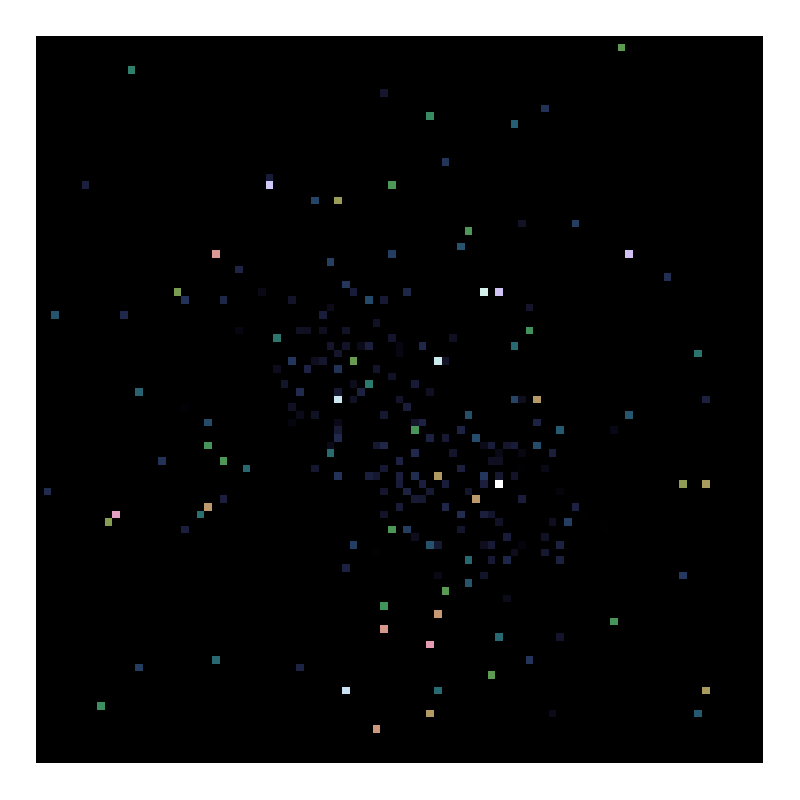
\includegraphics[width=1.00\linewidth, clip, trim= 0.25in 0.25in 0.25in 0.25in]{./chapters/05.pcdm/randomProblem/random_1k_block1.png}
		\caption{8k iterations}
		\label{pcdm:adaption:randomProblem:block11}
	\end{subfigure}
	\begin{subfigure}[b]{0.245\linewidth}
		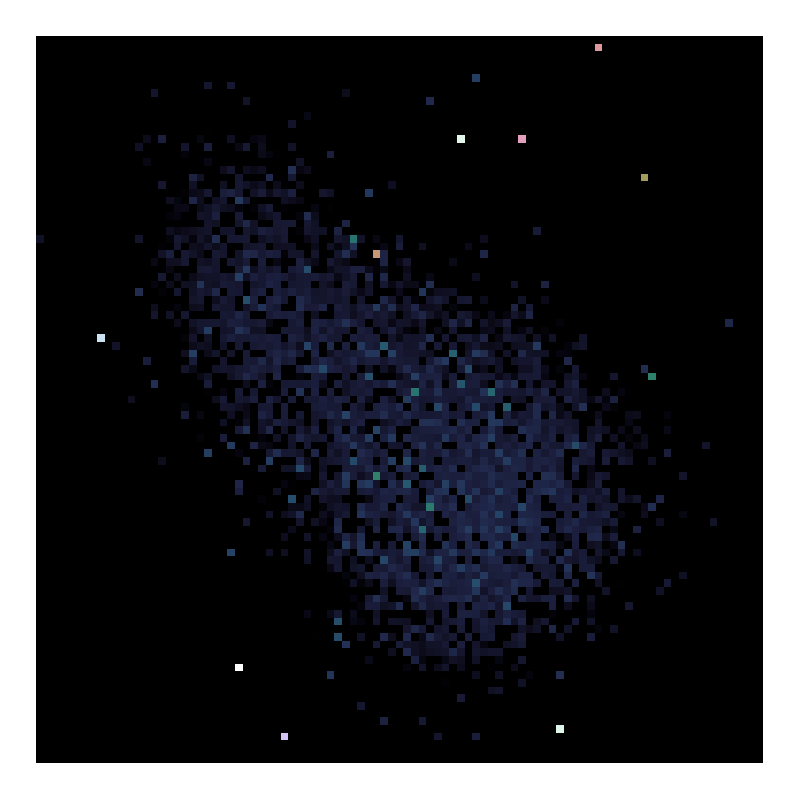
\includegraphics[width=1.00\linewidth, clip, trim= 0.25in 0.25in 0.25in 0.25in]{./chapters/05.pcdm/randomProblem/random_10k_block1.png}
		\caption{80k iterations}
		\label{pcdm:adaption:randomProblem:block12}
	\end{subfigure}
		\begin{subfigure}[b]{0.245\linewidth}
		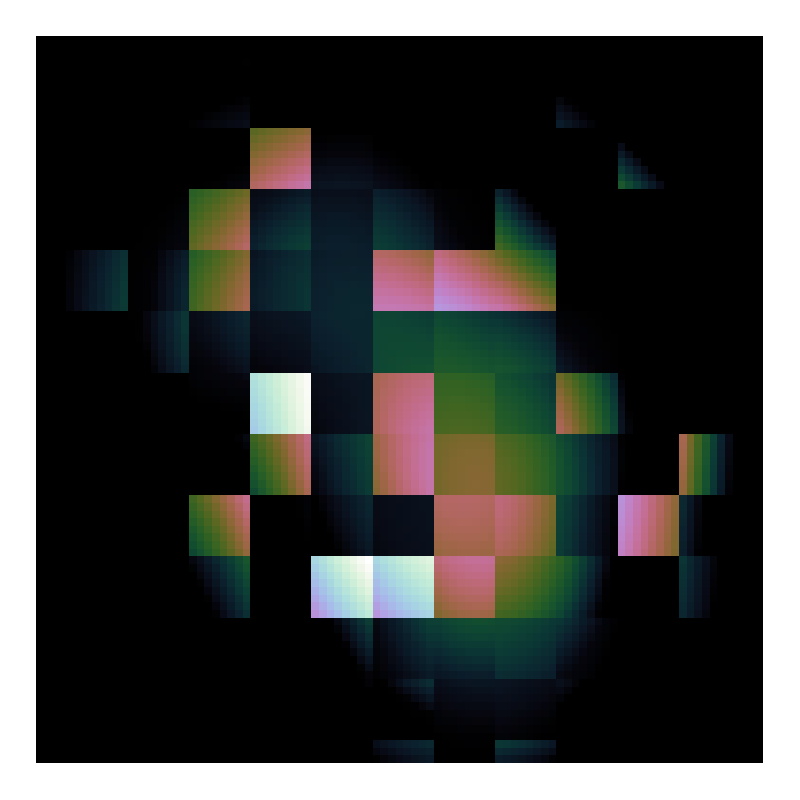
\includegraphics[width=1.00\linewidth, clip, trim= 0.25in 0.25in 0.25in 0.25in]{./chapters/05.pcdm/randomProblem/random_1k_block8.png}
		\caption{8k iterations, $8^2$ block}
		\label{pcdm:adaption:randomProblem:block81}
	\end{subfigure}
		\begin{subfigure}[b]{0.2405\linewidth}
		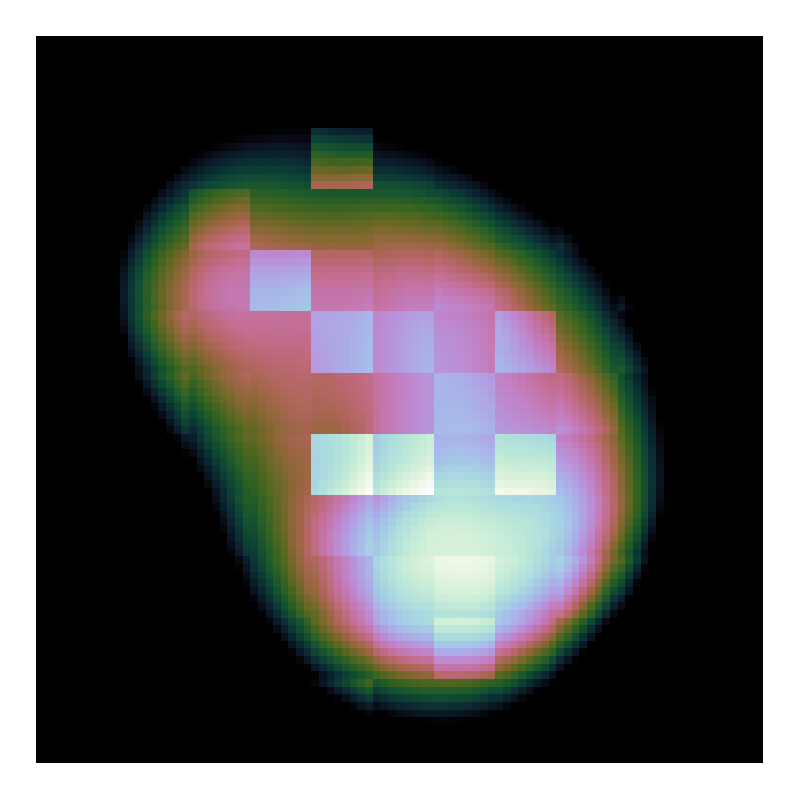
\includegraphics[width=1.00\linewidth, clip, trim= 0.25in 0.25in 0.25in 0.25in]{./chapters/05.pcdm/randomProblem/random_10k_block8.png}
		\caption{80k iterations, $8^2$ block}
		\label{pcdm:adaption:randomProblem:block82}
	\end{subfigure}
	\caption{Random parallel deconvolutions on the LMC N132D supernova remnant.}
	\label{pcdm:adaption:randomProblem}
\end{figure}

The Figure \ref{pcdm:adaption:randomProblem} shows the behaviour on the LMC observation. The reconstructions receive obvious artifacts from the random selection strategy. The blocks, which get selected in the first few iterations, keep their over-estimated values until we randomly select them again in later iterations. Other blocks in the neighborhood cannot be changed to a reasonable value until the algorithm has randomly selected the over-estimated blocks. That is why even after 80k iterations, the N132D supernova remnant gets only hinted at in Figure \ref{pcdm:adaption:randomProblem:block12}. Until the over-estimated blocks get selected again, the algorithm cannot do useful updates in that region.

This behavior is pronounced when we choose a block size of one pixel (i.e. we do not group pixels into blocks). Increasing the block size also increases our changes to select one of the over-estimated block again. But as we see in Figure \ref{pcdm:adaption:randomProblem:block82}, the same problem exists with larger block sizes, although less pronounced. After 80k iterations the N132D supernova remnant is visible, but a few random blocks still contain too much of the emission in that area.

The order in which we select blocks seems to be relevant in the deconvolution problem. A random selection strategy needs a prohibitive large number of iterations to converge. But we cannot simply switch out the selection strategy. The random selection strategy is at the core of the Parallel coordinate descent methods. Remember the ESO arises from the fact that we select $tau$ pixels uniformly at random. When we select $\tau$-pixels with a greedy strategy, we might break the ESO and may not converge.

To solve this behavior, we introduce the pseudo-random selection strategy:  We select a block at random, but greedily search in the neighborhood for the optimal block to optimize. The size of the neighborhood can be defined by the user. It is essentially a mix between a greedy and a random selection strategy. If we choose the neighborhood to be the whole image, we arrive at a greedy strategy. If we choose the neighborhood to be just one block, we are back at a random strategy. The mixture of the greedy and random strategy allows us to fix the problems with the pure random

We also introduced three heuristics that speed up the parallel deconvolution algorithm in practice: An active set heuristic, Restarting heuristic and a 'Minor' cycle.


\subsubsection{Active set heuristic}
The active set heuristic is typically used in cyclic coordinate descent: It chooses a subset of blocks, and optimizes the set until it converges. Then it chooses a  new set. We use the active set heuristic together with our pseudo-random selection strategy. A large portion of the blocks in the image will be zero. If we select blocks at pseudo-random, we are likely to select a block that will never contain non-zero values. The active set heuristic increases the likelihood that the pseudo-random strategy selects a relevant block. 

At the start of the parallel deconvolution algorithm, we iterate over all blocks. We add all blocks whose value can be changed to non-zero. During parallel iterations, the algorithm only selects blocks from the active set.

Note that the algorithm only adds blocks to the active set, which can be changed to a non-zero value at the start of deconvolution. Over several iterations, there may be blocks that are not in the active set, but are part of the optimal solution. This is remedied with a restarting heuristic.


\subsubsection{Restarting heuristic}
In accelerated gradient methods, like APPROX or (F)ISTA, restarting the acceleration can lead to a significant speedup\cite{fercoq2016restarting}. In our accelerated variant, restarting means we reset the acceleration variable $theta$ restart with the deconvolution, using the intermediate solution from the last iteration. Our accelerated deconvolution algorithm uses an active set. If we detect that important blocks are missing from the active set, we want to restart the deconvolution with a new active set. 

We implemented two restarting heuristics: One heuristic is based on Glasmachers et al.\cite{glasmachers2014coordinate} and restarts the algorithm when the acceleration likely benefits from it. The other heuristic was developed by us and restarts the when the active set is likely to be missing blocks. In our tests, we always needed to restart due to the active set, and never due to the heuristic by Glasmachers.

Our own restarting heuristic is based on the following idea: When the parallel deconvolutions start to converge before the currently best greedy step, we restart the algorithm with a new active set.

We introduce a new loop for the active set iteration. For each active set iteration, we execute several parallel deconvolution steps. For example, a single active set iteration may include 1000 parallel deconvolutions for each processor, running for $\tau * 1000$ iterations in total. Each processor updates the gradient maps and the reconstructed image asynchronously. We assume that after each active set iteration, we have landed at least once on the block that the greedy algorithm would have chosen in a single iteration.

At the end of each active set iteration, we check whether the parallel accelerated iterations converge faster than the currently best greedy step. If it does, we restart the parallel algorithm with a new active set.

\begin{lstlisting}
...
do
	lastMaxDiff = GetGreedyMaxBlockDiff(gradientsMapExplore, xExplore)
	parallelDiffFactor = 0
	for activeSetIteration in activeSetIterations
		
		//concurrent iterations
		maxParallelDiff = 0
		parallel for
			...
			diffBlock = optimalBlock - oldBlock
			...
			
			if(maxParallelDiff < diffBlock)
				maxParallelDiff = diffBlock
				
		//restarting heuristic
		if(parallelDiffFactor = 0)
			parallelDiffFactor = lastMaxDiff / maxParallelDiff
		
		currentMaxDiff = GetGreedyMaxBlockDiff(gradientsMapExplore, xExplore)
		activeSetInvalid = lastAbsMax / maxParallelDiff > parallelDiffFactor * 2
		activeSetInvalid = activeSetInvalid | currentMaxDiff > lastAbsMax & lastAbsMax / parallelDiffFactor > concurrentFactor
		if activeSetInvalid
			Restart()
			parallelDiffFactor = 0
		lastMaxDiff = currentMaxDiff
	..
while maxAbsDiff  < epsilon
\end{lstlisting}

After the first active set iteration, we check how close the maximum parallel update is to the best greedy step. The ratio of maximum greedy update and maximum parallel update should stay similar over the course of the algorithm, if the active set is valid. If the active set invalid, if it is missing important blocks, the algorithm will encounter ever smaller values for $maxParallelDiff$, while $lastMaxDiff$ does not decrease significantly over the active set iterations. In that case, the ratio between $lastMaxDiff / maxParallelDiff$ sharply increases, and we restart the algorithm.

We have two similar conditions on which we flag the active set as invalid. If the ratio of $lastMaxDiff / maxParallelDiff$ is twice as big as the ratio of the first active set iteration, we restart the algorithm. The second condition is based on the observation that the $currentMaxDiff$ may increase from active set iteration to active set iteration. In this case, we are likely missing important blocks in the active set and we restart more aggressively: If the ratio $lastMaxDiff / maxParallelDiff$ bigger than the ratio of the first active set iteration.


\subsubsection{Re-introduction of a 'Minor' cycles}
As we will demonstrate in the next section, the parallel coordinate descent deconvolution algorithm benefits significantly from our $PSF$ approximation. The drawback of our $PSF$ approximation is that it needs more major cycles to converge. We re-introduce a similar minor cycle to the Clark CLEAN algorithm \cite{clark1980efficient}, and reduce the number of necessary major cycles.

The CLEAN algorithm developed by Clark also uses only a fraction of the $PSF$ during CLEAN deconvolutions. After a number of iterations, the residuals of the Clark algorithm are inaccurate, and it resets the residuals with the full $PSF$.

We use a similar idea: We run our parallel coordinate descent deconvolution algorithm, and retrieve the intermediate solution. We then decide whether we reset the residuals using the full $PSF$ (the 'minor' cycle), or we use the major cycle.

Resetting the residuals with the full $PSF$ is done as follows:

\begin{lstlisting}
residuals = iFFT(Gridding(visibilities))  	//Major cycle
x = deconvolve(residuals, Cut(PSF)) 		//Deconvolve with approximate PSF
residuals_minor = residuals - iFFT(FFT(x) * FFT(PSF))
\end{lstlisting}

We convolve the intermediate solution $x$ with the $PSF$ in Fourier space, and subtract the result from the original residuals from the major cycle. This allows us to use fewer major cycles when we use an aggressive $PSF$ approximation.

The question only question that remains is, when to use a major cylce or a 'minor' cycle. Remember from Section \ref{gradients}, we introduced a heuristic based on the $PSF$ sidelobe: When we deconvolve using only a fraction of the full $PSF$, we leave sidelobes in the residual image. In each major cycle, we can only run the deconvolution algorithm up to a certain point, before we include $PSF$ sidelobes in the reconstructed image. 

In Section \ref{gradients} solved this by estimating a minimum regularization parameter $\lambda$ for each major cycle. Now with the addition of a 'minor' cycle, we use the same heuristic twice: We have two minimum regularization parameters, $\lambda_{minor}$ and $\lambda_{major}$. We use the minor cycle, as long as  $\lambda_{minor}$ is larger than  $\lambda_{major}$. Otherwise, we start a new major cycle. In total, the major and 'minor' cycle for our parallel coordinate descent algorithm is implemented as follows:

\begin{lstlisting}
residualVis = visibilities
x = new Array[,]

for each cycle in Range(0, maxMajorCycles)
	residuals = iFFT(Gridding(residualVis))
	residualsMinor = residuas
	
	lambdaMajor = Estimate(residuals, PSF, 2)
	lambdaMinor = 0
	
	do
		lambdaMinor = Estimate(residualsMinor, PSF, psfFraction)
		lambdaMinor = Max(lambdaMinor, lambdaMajor)
		
		x_current = deconvolve(residuals, Cut(PSF, psfFraction))
		x + = x_current
		residuals_minor = residuals - iFFT(FFT(x) * FFT(PSF))
	while(lambdaMajor < lambdaMinor)
	
	modelVis = DeGridding(FFT(x))
	residualVis = visibilities - modelVis
\end{lstlisting}

Estimating $\lambda_{minor}$ is identical to the heuristic developed in Section \ref{gradients}. We use the maximum sidelobe of the $PSF$ which is not contained in the cutout used for deconvolution. Estimating $\lambda_{major}$ is more difficult: In theory, we use the full $PSF$, and do not have a sidelobe outside the cutout. However, we also know that the full $PSF$ is only an approximation (remember: the $w$-term changes the $PSF$ slightly for all pixels in the image). For the parameter $\lambda_{major}$, we simply use the maximum sidelobe outside of the $\frac{1}{2}$ cutout.


\subsection{Tests on the LMC Observation}\label{pcdm:results}
We have shown the parallel coordinate descent algorithm in two variants: With gradient acceleration and without. We developed several heuristics, which includes a set of tuning parameters. In this section, we test our parallel coordinate descent algorithm on the MeerKAT LMC observation. We test the tuning parameters, and show how much our algorithm benefits from the $PSF$ approximation method.

In this test, we measure the wall-clock time of only the deconvolution. The wall-clock time of the Major- and 'Minor' cycle are excluded. Again, we calculate the value of the objective function. We compare different parameters of our parallel coordinate descent algorithm, trying to get the shortest convergence time.

\subsubsection{$PSF$ approximation}
First, we test the effect of our $PSF$ approximation method. We test different $PSF$ cutouts of our parallel coordinate descent algorithm with gradient acceleration. We use $\tau = 8$ processors with our asynchronous implementation.

Figure \ref{pcdm:results:psf} shows the result of our parallel coordinate descent algorithm with different $PSF$ fractions, combined with the ESO and the total seconds needed to converge. The $y$-axis shows the objective value, and the $x$-axis shows the elapsed seconds. Note that the axis of the figure are logarithmic. The 'kinks' in the lines are due to either the Major or the 'Minor' cycle resetting the residuals (remember: we do not include the wall-clock time of the Major or 'Minor' cycle in this test).

\begin{figure}[h]
	\centering
	\begin{subfigure}{0.6\linewidth}
		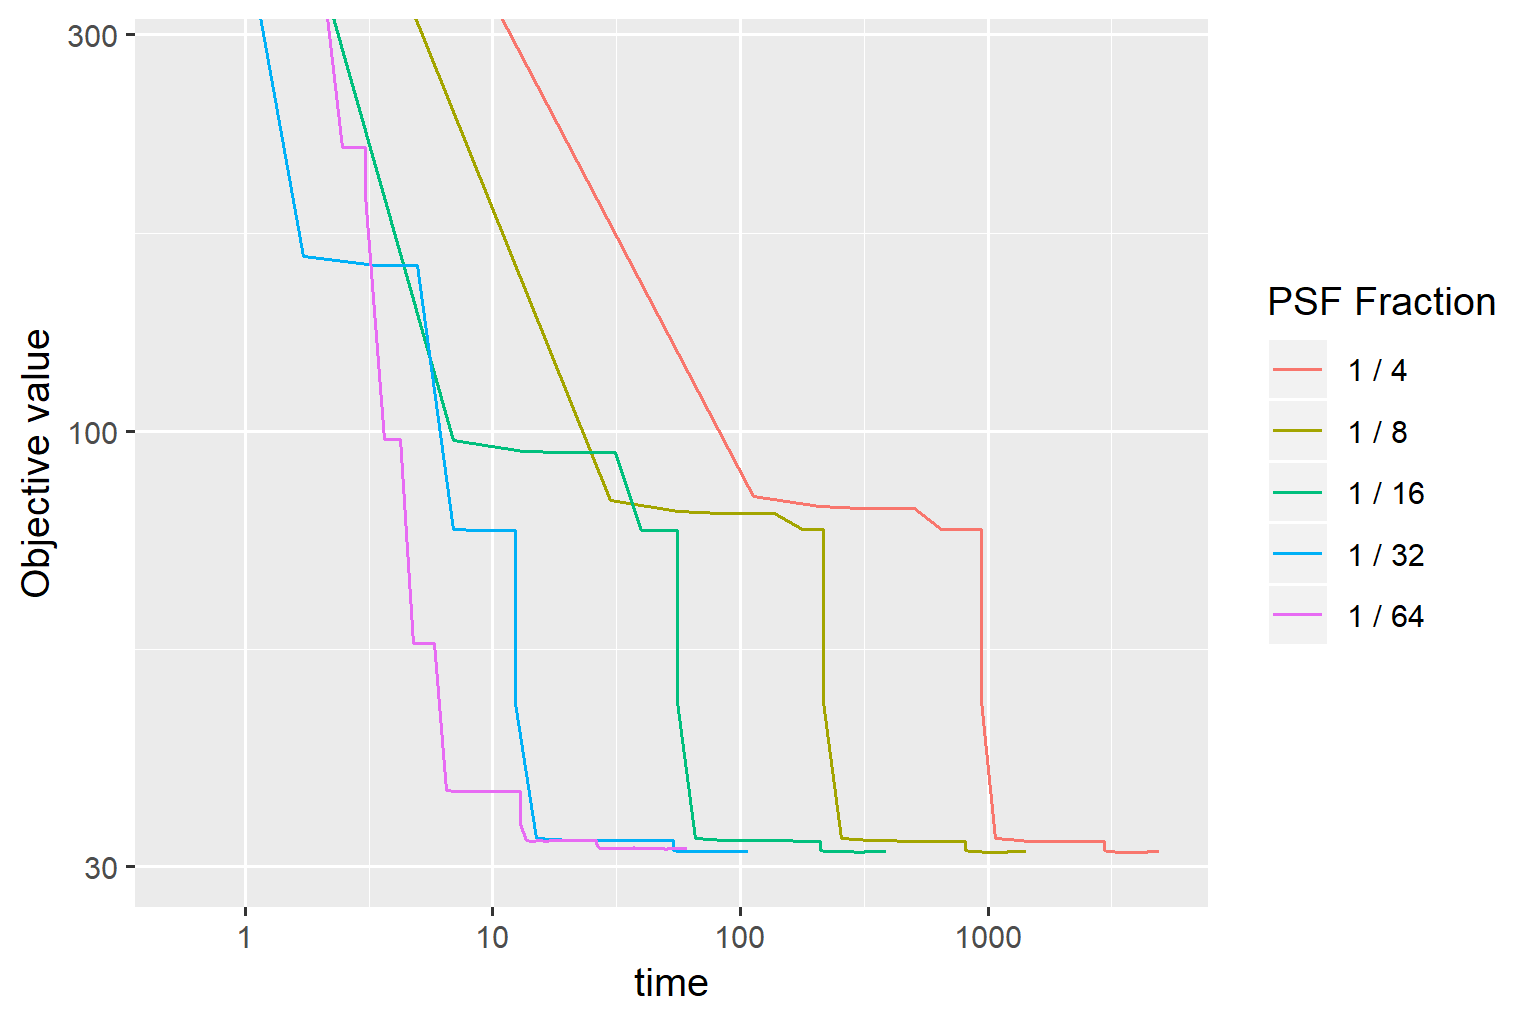
\includegraphics[width=1.0\linewidth]{./chapters/05.pcdm/parameters/psfSize.png}
	\end{subfigure}
	\begin{subfigure}{0.35\linewidth}
		\begin{tabular}{c | r | r}
			PSF & ESO & Total seconds \\ \hline
			1 / 4 & 2.750 & 4941 \\
			1 / 8 & 1.437 & 1433 \\
			1 / 16 & 1.109 & 390 \\
			1 / 32 & 1.027 & 108 \\
			1 / 64 & 1.001 & 61 \\
		\end{tabular}
	\end{subfigure}
	\caption{Convergence times with $PSF$ approximation}
	\label{pcdm:results:psf}
\end{figure}

Clearly, the parallel coordinate descent algorithm benefits from our $PSF$ approximation method. If we use $\frac{1}{32}$ of the full $PSF$, the parallel coordinate descent algorithm spends a total of 108 seconds in to deconvolve the image. For comparison, the serial coordinate descent algorithm with $PSF$ approximation takes roughly 1400 seconds, or 23 minutes.

As expected, with increasing $PSF$ approximation, we get an ESO which is ever closer to 1. Remember: An ESO of 1 means that each processor in the parallel coordinate descent algorithm can has the same step size as the serial coordinate descent algorithm. With an approximation of $\frac{1}{32}$ and 8 parallel processors, the ESO is only marginally larger than 1. This suggests that the parallel coordinate descent algorithm may be sped up further with additional processors.

Note that the speedup from fraction $\frac{1}{4}$ to $\frac{1}{8}$ is roughly a factor of $3.5$. The same holds true for the speedup of $\frac{1}{8}$ to $\frac{1}{16}$, and $\frac{1}{16}$ to $\frac{1}{32}$. The $PSF$ cutout from  $\frac{1}{8}$ to  $\frac{1}{16}$ four times fewer pixels. This suggest the speedup may be due to the reduced conflicts in the asynchronous update of the gradient map. With a smaller $PSF$ we reduce the change of several threads updating the same location in the gradient map, and we spend more time in the deconvolution itself.

For the rest of this project, we will use a $PSF$ approximation of $\frac{1}{32}$ for the parallel coordinate descent algorithm. The $\frac{1}{64}$ approximation is faster in this tests, but needs more 'Minor' cycles (Which were excluded from the wall-clock time). Including the time spent in the 'Minor' cycle, the $\frac{1}{32}$ approximation is the fastest overall.


\subsubsection{Block size}
The parallel coordinate descent algorithm can group several pixels in blocks, and optimize the blocks of pixels in parallel. It is not clear if grouping the pixels in blocks results in shorter convergence times. We test different block sizes in Figure \ref{pcdm:results:block}, all using the same $PSF$ approximation of $\frac{1}{32}$. We tested out block size of $1^2$ (every block contains a single pixel) up to a block size of $8^2$:

\begin{figure}[h]
	\centering
	\begin{subfigure}{0.6\linewidth}
		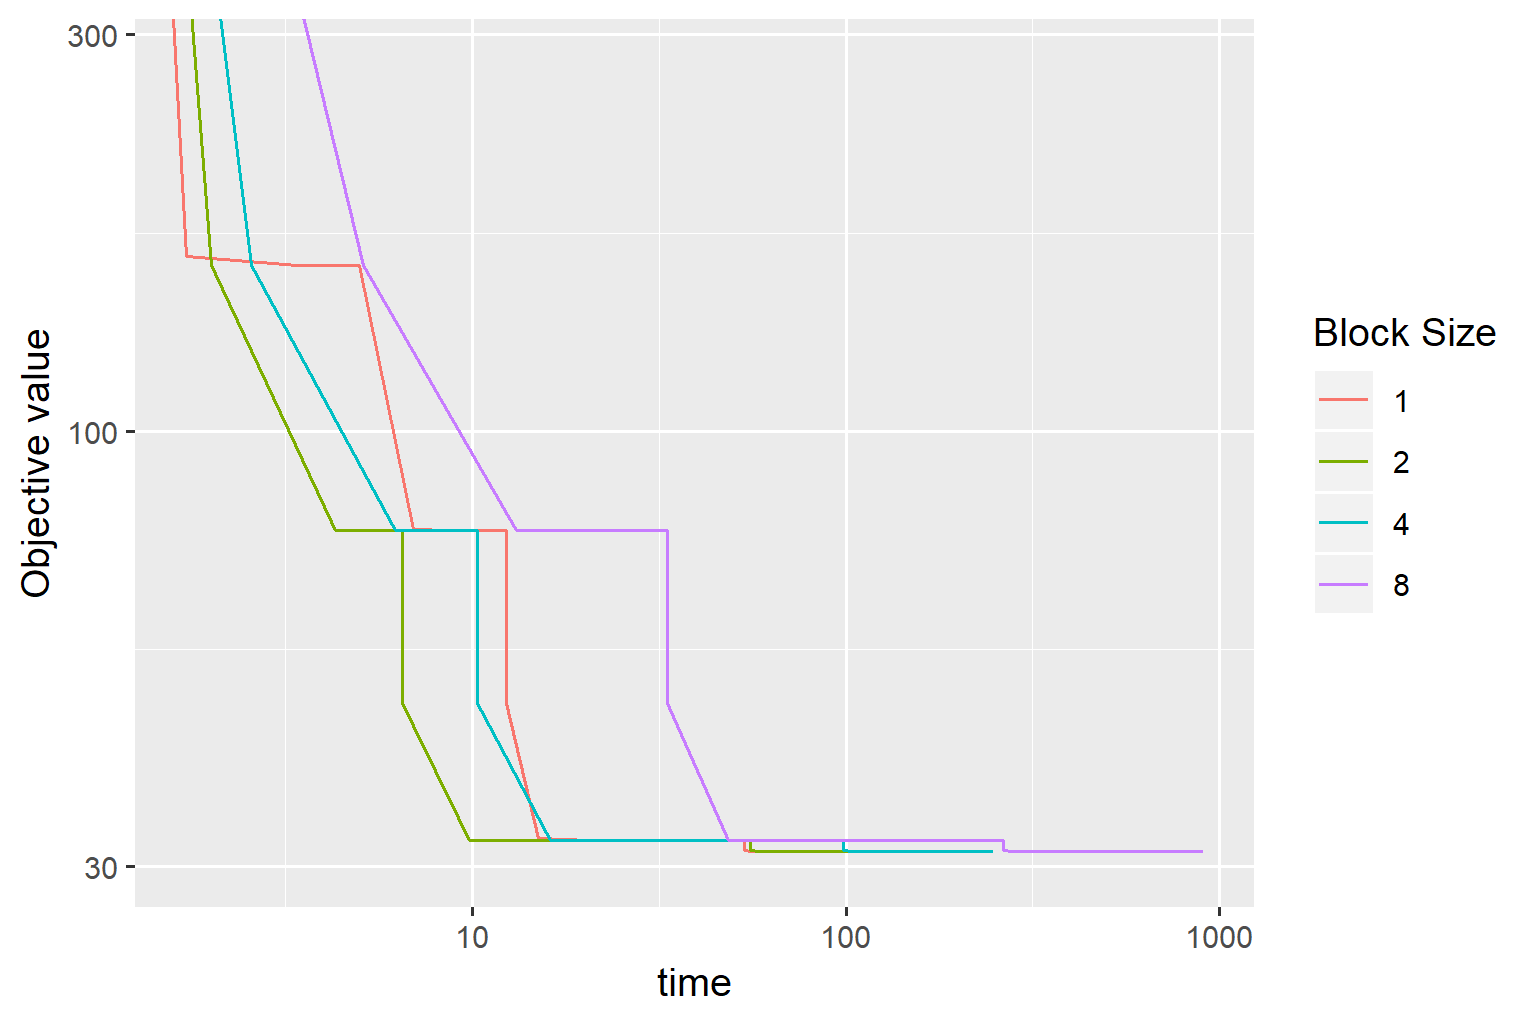
\includegraphics[width=1.0\linewidth]{./chapters/05.pcdm/parameters/blockSize.png}
	\end{subfigure}
	\begin{subfigure}{0.35\linewidth}
		\begin{tabular}{c | r}
			Block Size & Total seconds \\ \hline
			$1^2$ & 108 \\
			$2^2$ & 103 \\
			$4^2$ & 248 \\
			$8^2$ & 905 \\
		\end{tabular}
	\end{subfigure}
	\caption{Convergence times with different block sizes}
	\label{pcdm:results:block}
\end{figure}

The larger block sizes of $4^2$ and $8^2$ are significantly slower to converge than a block size of $1^2$. Only a block size of $2^2$ is slightly faster. Interestingly though, the parallel coordinate descent algorithm is faster to arrive at intermediate results with the block sizes $2^2$ and $4^2$. This suggests that the parallel coordinate descent algorithm may benefit starting out from larger block sizes, and gradually reducing the block size over several major cycle iterations.

However, two factors lead to the decision to simply use a block size of $1^2$ for all major cycle iterations: First, the block size is likely connected to the image resolution. An effective heuristic that starts with larger blocks may become difficult to develop for general observations. Secondly, the parallel coordinate descent implementation becomes more complicated when it has to account for different block sizes. An implementation with a block size of only $1^2$ is shorter and simpler.

For the rest of this project, we use a block size of $1$, meaning every thread is minimizing a single pixel.


\subsubsection{Pseudo-random strategy}
We discussed in Section \ref{pcdm:adaption}, a random block selection strategy seems to perform badly on the deconvolution problem. We created the pseudo-random strategy, which selects a block at random, but searches in it's neighborhood for the optimal block to optimize. It is a mixture between a random and a greedy selection strategy.

But the pseudo-random strategy introduces a new tuning parameter, which we call the 'search factor'. A search factor of 0 says that after a random block has been selected, we search 0\% of the neighboring blocks in the active set. It is identical to a pure random selection strategy. A search factor of 1.0 says that after a random block has been selected, we search 100\% of its neighbors in the active set. For example, if we have 256 blocks with 8 threads, a search percentage of 1.0 selects a random block and looks at 32 blocks in its neighborhood. A search percentage of 100\% is identical to a greedy strategy, where each thread searches its part of the active set.

Our parallel coordinate descent algorithm needs a search percentage larger than 0. We compare different search percentages in Figure \ref{pcdm:results:search}.

\begin{figure}[h]
	\centering
	\begin{subfigure}{0.6\linewidth}
		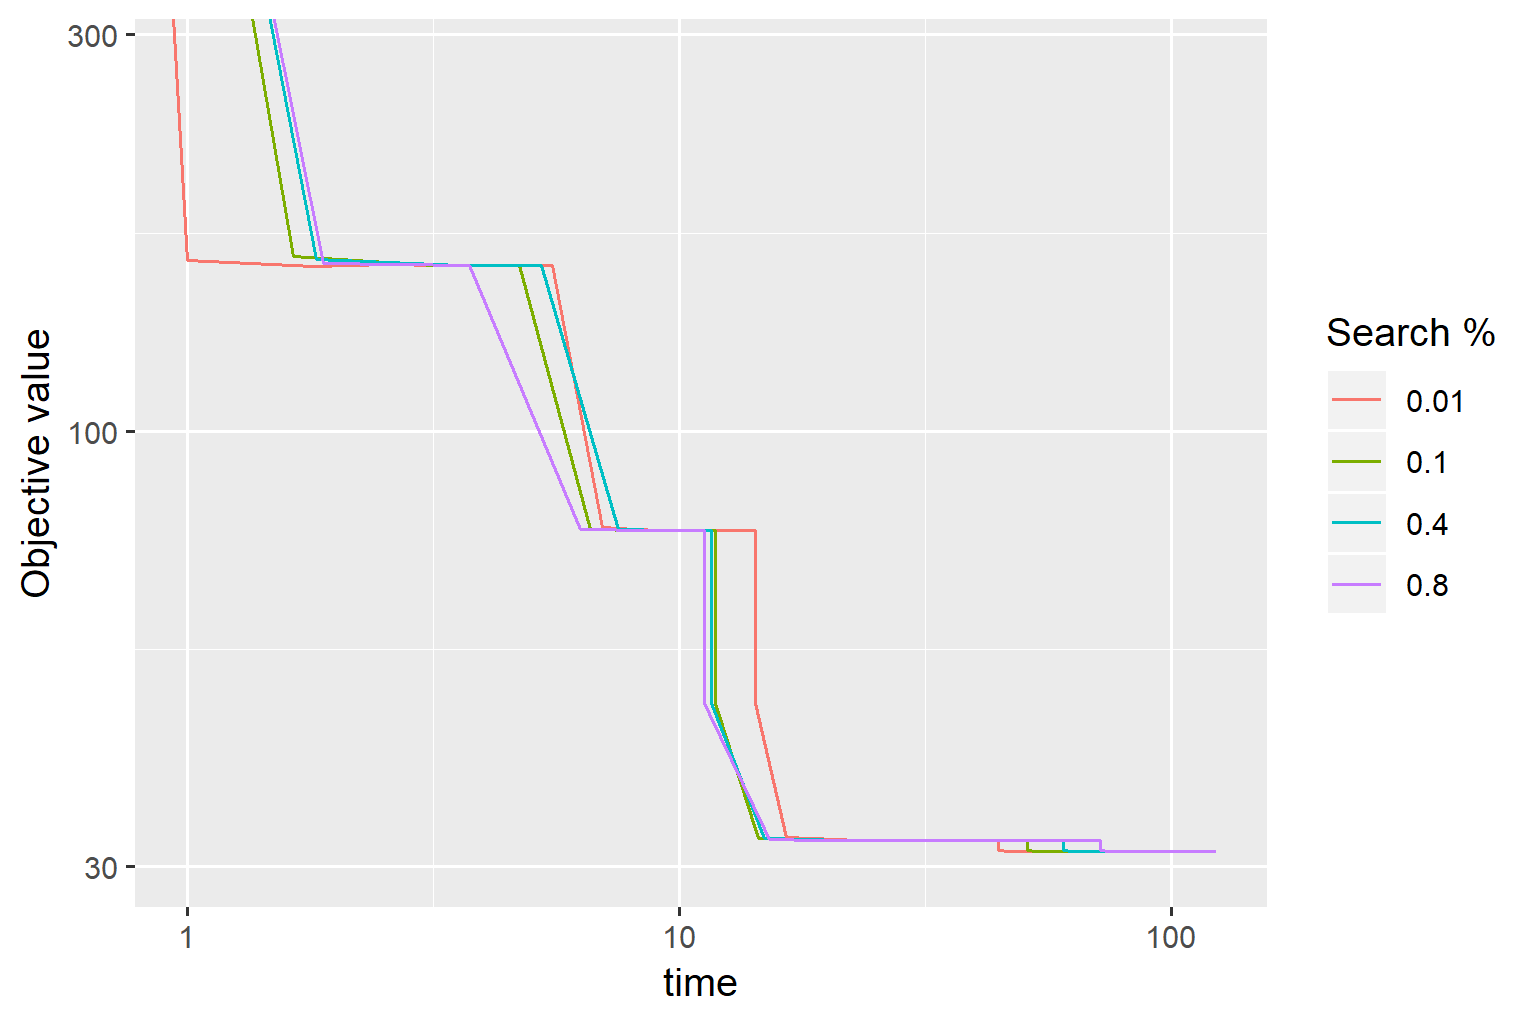
\includegraphics[width=1.0\linewidth]{./chapters/05.pcdm/parameters/searchPercent.png}
	\end{subfigure}
	\begin{subfigure}{0.35\linewidth}
		\begin{tabular}{c | r}
			Search Factor & Total seconds \\ \hline
			0.01 & 110 \\
			0.1 & 106 \\
			0.2 & 104 \\
			0.4 & 112 \\
			0.8 & 134 \\
		\end{tabular}
	\end{subfigure}
	\caption{Convergence times with different search percentages.}
	\label{pcdm:results:search}
\end{figure}

According to this test, the search factor tuning parameter influences the convergence speed, but tuning it does not lead to a significant speedup. A value between 0.01 and 0.4 leads to a similar wall-clock time. It is only when the parameter is set close to 1 (close to fully greedy) where we see a significant increase in wall-clock time.

Based on this test, we fixed the search percentage tuning parameter to a value of 0.1 for all tests in this project. It was enough to alleviate the problems a pure random strategy introduces in the deconvolution problem (discussed previously in Section \ref{pcdm:adaption}).

However, we do not know whether this parameter generally has a small influence on convergence speed, or if it is merely due to the LMC observation we used for this project. To answer this question, we need further tests on diverse observations.


\subsubsection{Acceleration}
Lastly, we test whether the parallel coordinate descent algorithm is faster with or without gradient acceleration. The accelerated variant needs two versions of the gradient map, which get updated asynchronously with compare-exchange operations. Figure \ref{pcdm:results:acc} compares the accelerated and non-accelerated parallel coordinate descent algorithm.

\begin{figure}[h]
	\centering
	\begin{subfigure}{0.6\linewidth}
		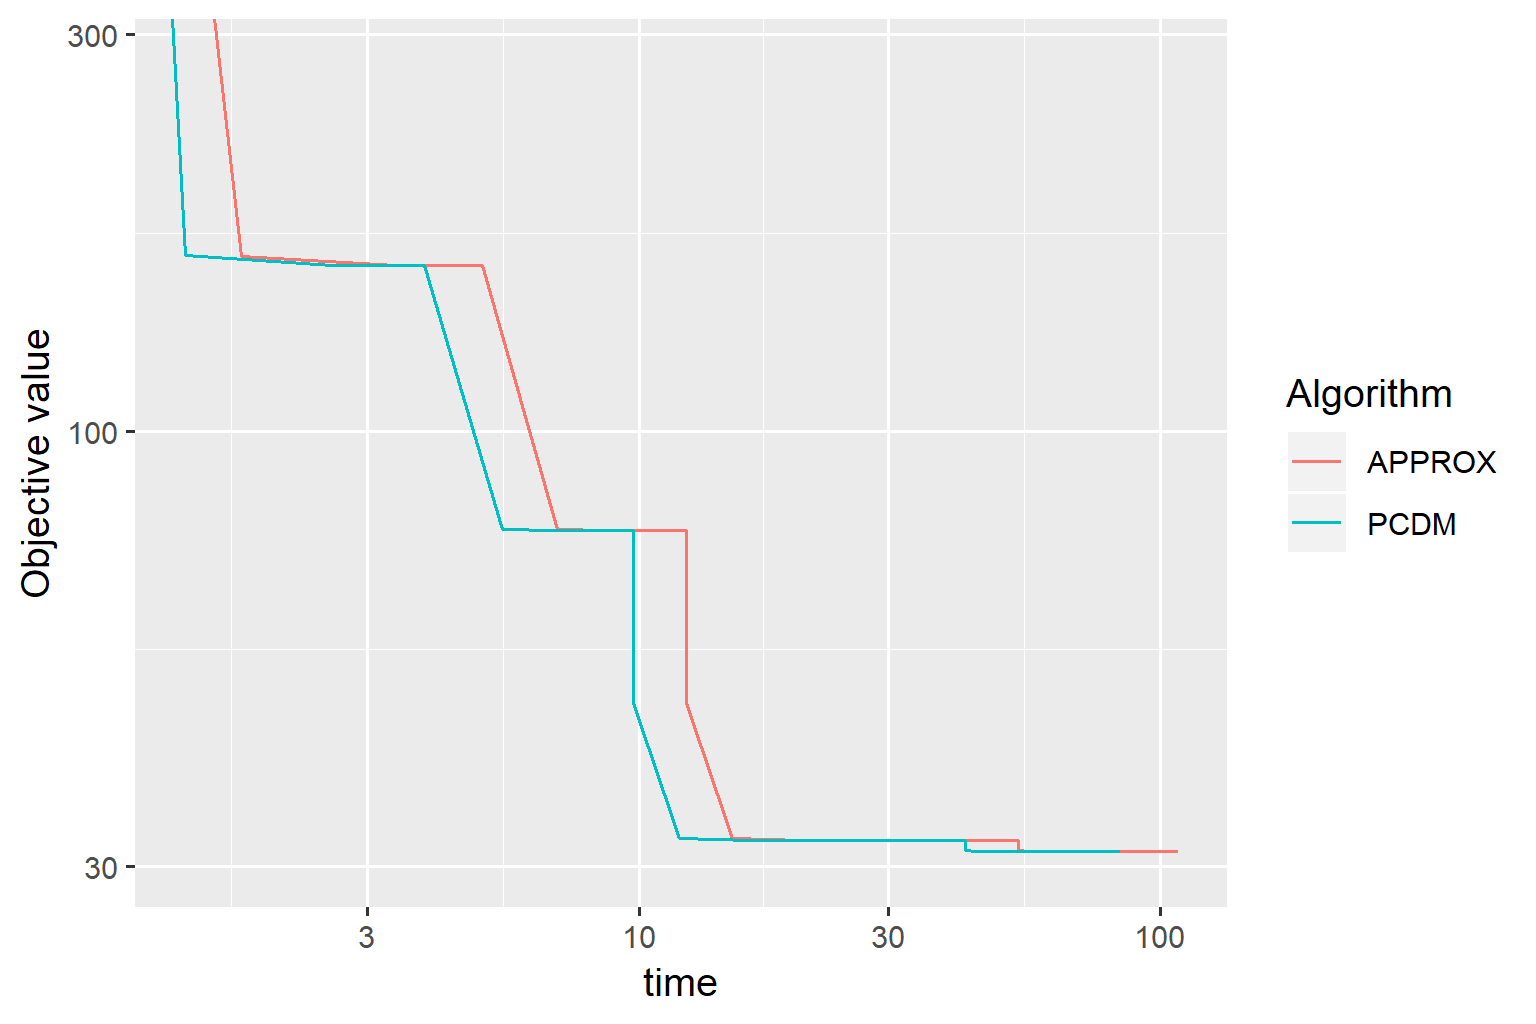
\includegraphics[width=1.0\linewidth]{./chapters/05.pcdm/parameters/acceleration.png}
	\end{subfigure}
	\begin{subfigure}{0.35\linewidth}
		\begin{tabular}{c | c}
			Method & Total seconds \\ \hline
			With Acceleration & 108 \\
			Without Acceleration & 84 \\
		\end{tabular}
	\end{subfigure}
	\caption{Convergence time with or without gradient acceleration.}
	\label{pcdm:results:acc}
\end{figure}

The accelerated variant is significantly slower in every part of the algorithm. Our hypothesis is that the two gradient maps necessary for the acceleration also increase the cost of synchronization.

Furthermore the accelerated variant has additional run time costs which were not measured in this test: It has to create a copy of the gradient map and the reconstructed image for the acceleration. Meaning this test shown in Figure \ref{pcdm:results:acc} is biased in favor of the accelerated variant, yet it is still slower.


\subsection{Comparison to the serial coordinate descent algorithm}
In the previous section, we tested various tuning parameters of the parallel coordinate descent algorithm. In this section, we compare the serial coordinate descent algorithm with the final, simplified parallel coordinate descent algorithm.

We took the lessons from the tests and implemented a simplified parallel coordinate descent algorithm. It does not use gradient acceleration, and cannot group pixels into blocks. Each thread can only minimize a single pixel in parallel in each iteration. As we will see shortly, the simplified parallel coordinate descent implementation is significantly faster than the previous implementation.

In this test, we compare the wall-clock time spent on the deconvolution algorithm. The time we measure here does not include the Major cycle. For the parallel coordinate descent algorithm, this means we also measure the time spent in the 'Minor' cycle for the parallel coordinate descent algorithm (which was excluded in the previous tests).

We use the same hardware as in the tests of Section \ref{results:LMC}. The table \ref{pcdm:comp:table} shows the comparison between the serial and parallel coordinate descent algorithm. The parallel coordinate descent algorithm achieved a speedup factor of roughly $20$. While the serial coordinate descent algorithm takes over 20 minutes to deconvolve the image, the parallel coordinate descent algorithm takes less than two minutes in total.
%hardware

\begin{table} [h]
	\centering
	\begin{tabular}{c | c | r | r | c}
		Algorithm &  $PSF$  & Major Cycles & Total Seconds in Deconvolution & Speedup factor\\ \hline
		Serial CD & $\frac{1}{16}$ & 4 & 1486 & --\\
		Parallel CD & $\frac{1}{32}$ & 5 & 75 & $\approx 20$ \\
	\end{tabular}
	\caption{Speedup comparison of the serial and parallel coordinate descent algorithm. Both algorithms were compared on an Intel Xeon E3-1505M with 8 logical cores.}
	\label{pcdm:comp:table}
\end{table}

This parallel coordinate descent implementation is even faster than the implementation tested in the previous Section \ref{pcdm:results}. This implementation is simpler because it does not account for different block sizes. Each processor deconvolves a single pixel in parallel. The simplification leads to another decrease in wall-clock time.

The total deconvolution time of the parallel coordinate descent algorithm is in the range of the CLEAN algorithm. An exact comparison was not possible in this project. We did not implement the CLEAN algorithm in our .Net Core pipeline. However, the serial coordinate descent algorithm has an almost identical structure to the standard CLEAN algorithm, and we use this fact to get a rough comparison to CLEAN: The multi-scale CLEAN algorithm required 15'000 iterations to converge on the LMC observation. 15'000 serial coordinate descent iterations on the same hardware take approximately 230 seconds, which is more than the parallel coordinate descent algorithm needed.

The serial coordinate descent algorithm is significantly slower than the parallel algorithm. However, it requires one major cycle less than the parallel algorithm to arrive at a similar reconstruction. The Figure \ref{pcdm:comparison:figure} compares the reconstruction of the two algorithms of the LMC observation.

\begin{figure}[h]
	\centering
	\begin{subfigure}{0.45\linewidth}
		\centering
		Serial CD
		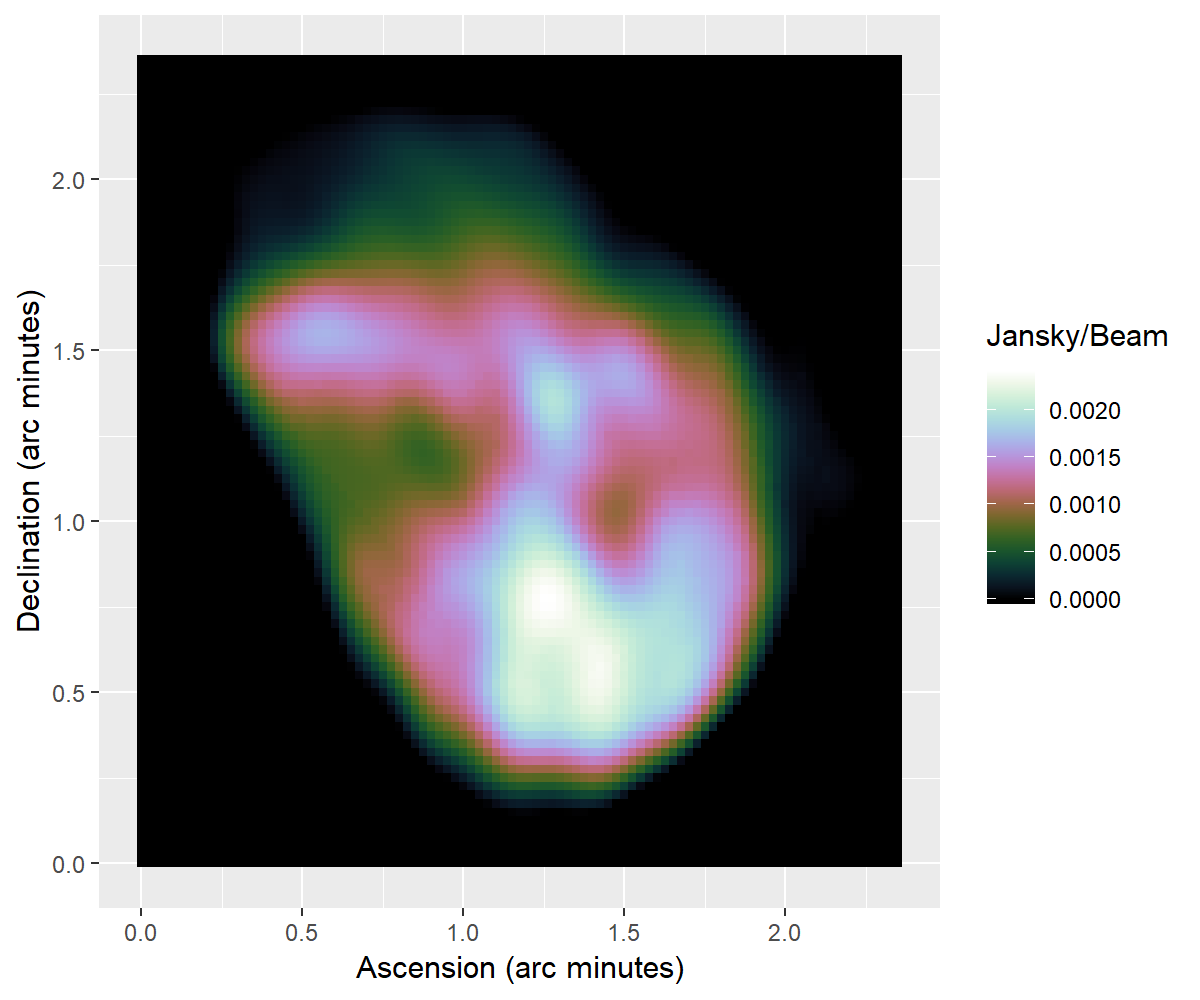
\includegraphics[width=1.0\linewidth]{./chapters/05.pcdm/comparison/SerialCD-N132.png}
	\end{subfigure}
	\begin{subfigure}{0.45\linewidth}
		\centering
		Parallel CD
		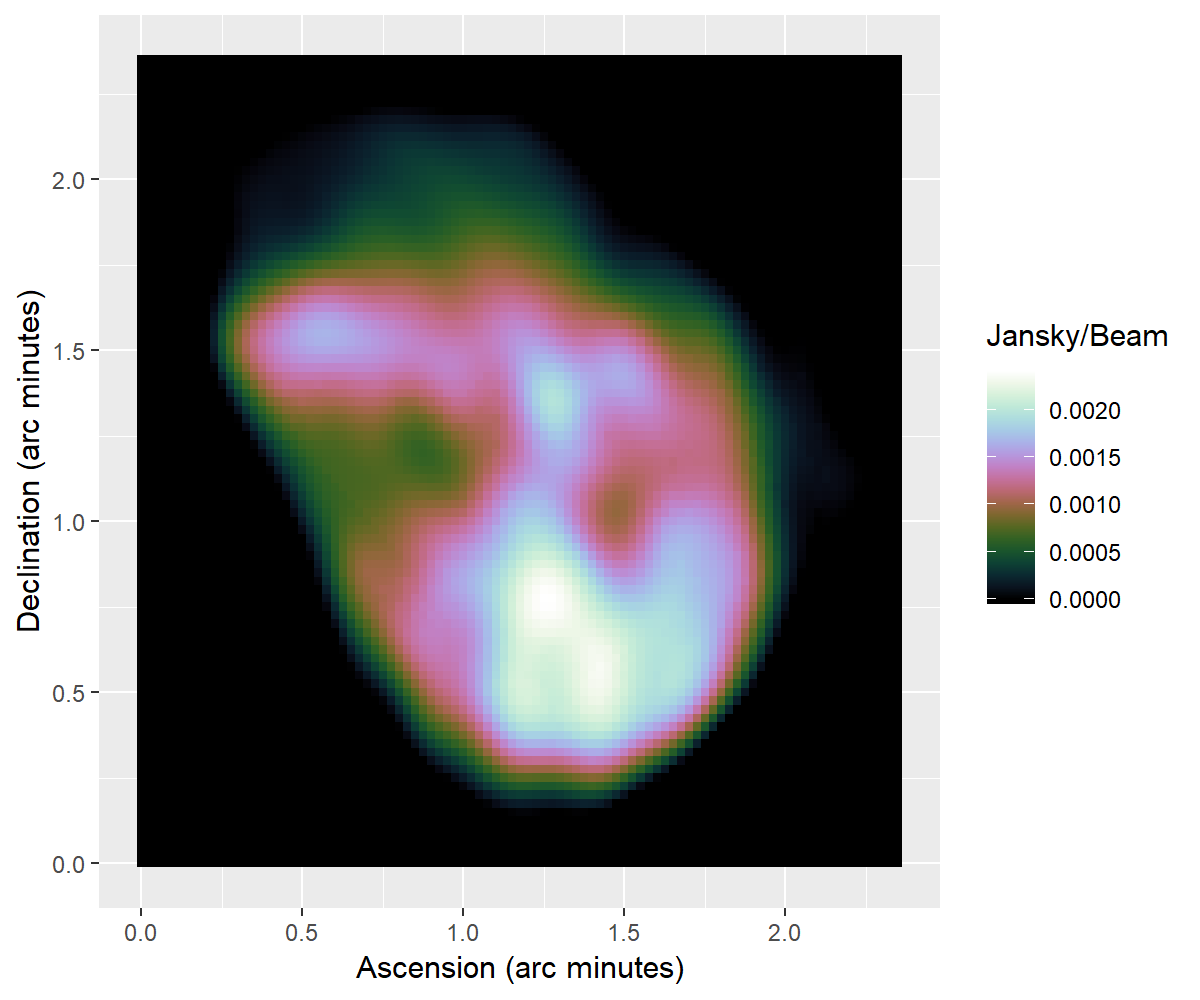
\includegraphics[width=1.0\linewidth]{./chapters/05.pcdm/comparison/SerialCD-N132.png}
	\end{subfigure}
	\\
	\begin{subfigure}{0.45\linewidth}
		\centering
		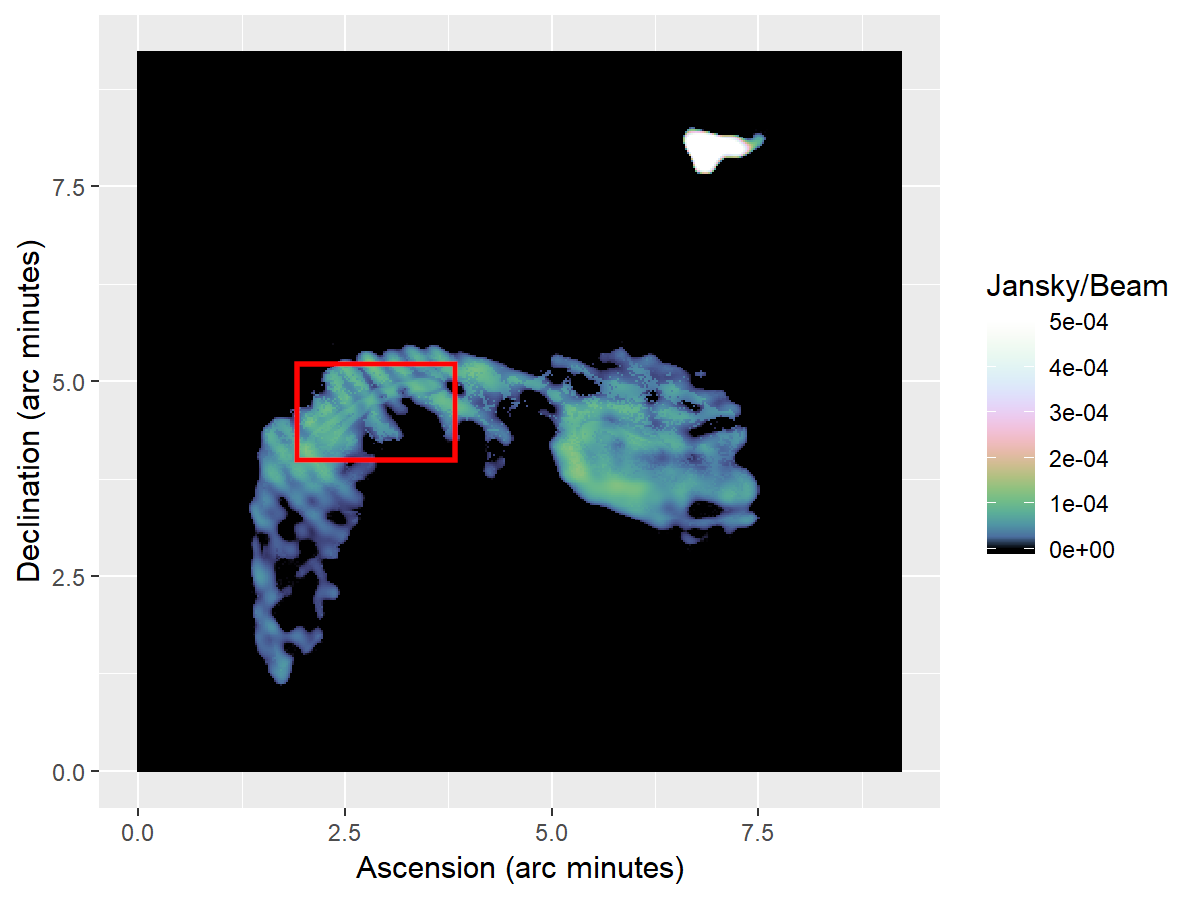
\includegraphics[width=1.0\linewidth]{./chapters/05.pcdm/comparison/SerialCD-Calibration2.png}
	\end{subfigure}
	\begin{subfigure}{0.45\linewidth}
		\centering
		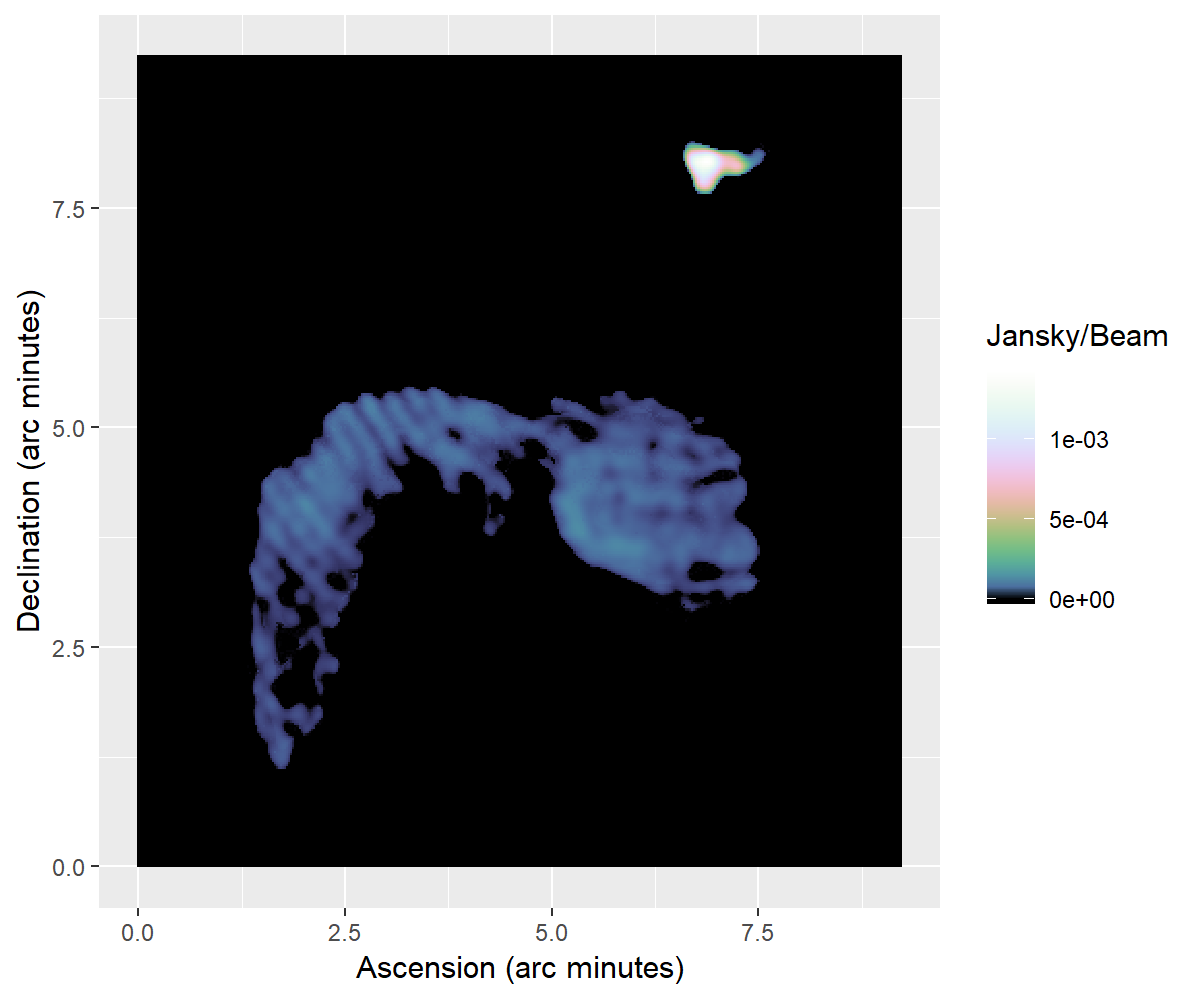
\includegraphics[width=1.0\linewidth]{./chapters/05.pcdm/comparison/PCDM-Calibration.png}
	\end{subfigure}

	\caption{Comparison of the serial and parallel coordinate descent reconstruction of the LMC observation.}
	\label{pcdm:comparison:figure}
\end{figure}

Both algorithms arrive at the same reconstruction. Both can super-resolve the N132D supernova-remnant, and have artifacts due to calibration errors. But the serial coordinate descent algorithm has left artifacts from the previous major cycles in the reconstruction: The red rectangle highlights a structure, which was added in a previous major cycle with the implicit path regularization. In a previous major cycle, only the highlighted structure was added. The next major cycle then added all the surrounding structure, including the "waves" from the calibration error. But the serial coordinate descent algorithm did not have enough iterations to properly integrate the old structure from the previous major cycle, leaving a "ghost" structure behind.

The serial coordinate descent can correct the artifact, but it either needs more iterations, or even another major cycle. In either case the serial coordinate descent algorithm needs more computing resources.

The parallel coordinate descent algorithm on the other hand does not contain the "ghost" structure. In a previous major cycle, the parallel algorithm has added a similar structure, but it was able to properly integrate it in the final reconstruction. We suspect this difference is due to the different number of pixels minimized: The reconstruction of the parallel algorithm is the result of roughly half a million single pixel minimizations, while the serial algorithm was had performed roughly 100 thousand single pixel minimizations. The parallel algorithm had more iterations to integrate the structures detected from previous cycles.

Overall the reconstruction of the serial and parallel coordinate descent algorithms are similar. On the LMC dataset, the parallel algorithm was able to reconstruct a slightly superior reconstruction within a fraction of the total run time of the serial algorithm.


\subsection{Scalability of the parallel coordinate descent algorithm}\label{pcdm:scale}
The parallel coordinate descent algorithm out-performs the serial algorithm significantly on personal computing hardware. Lastly, we want to investigate how the parallel algorithm behaves when we increase the number of asynchronous processors.

Our parallel coordinate descent algorithm is based on PCDM\cite{richtarik2016parallel}. PCDM has been extended for the distributed setting as Hydra\cite{richtarik2016distributed}, and in its accelerated variant as Hydra$^2$\cite{fercoq2014fast}. Extending our parallel coordinate descent algorithm to the distributed setting was not possible in the time frame of this project. But if the parallel algorithm should be distributed in the future, we can apply the methods developed for Hydra and Hydra$^2$.

We test the parallel coordinate descent algorithm on a shared memory system (all processors have access to the same main memory), and test how the algorithm behaves for larger number of processors. Figure \ref{pcdm:scalability:proc} shows the results. The first graph shows the total speedup, the second plot shows the total number of iterations needed, and the last plot shows the ESO for increasing number of processors.

\begin{figure}
	\centering
	\begin{subfigure}{0.30\linewidth}
		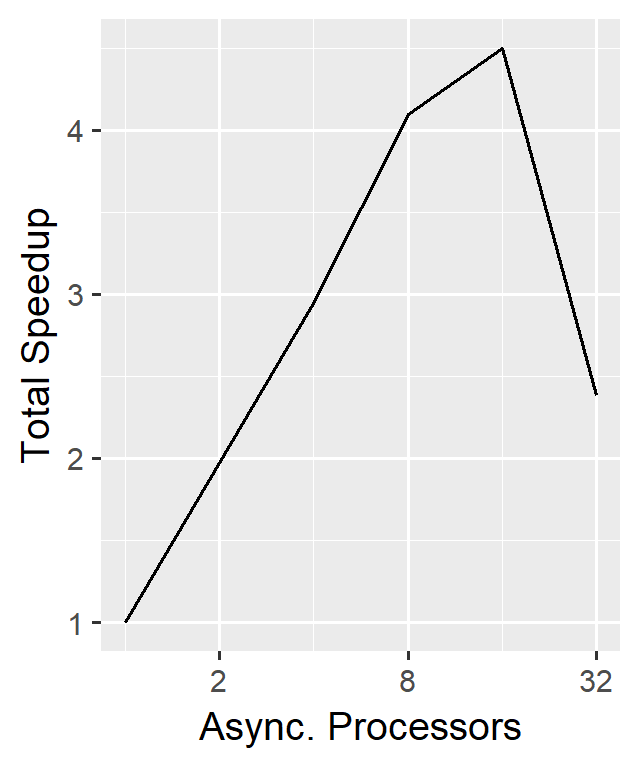
\includegraphics[width=1.0\linewidth]{./chapters/05.pcdm/scalability/speedup_pcdm_time.png}
	\end{subfigure}
	\begin{subfigure}{0.30\linewidth}
		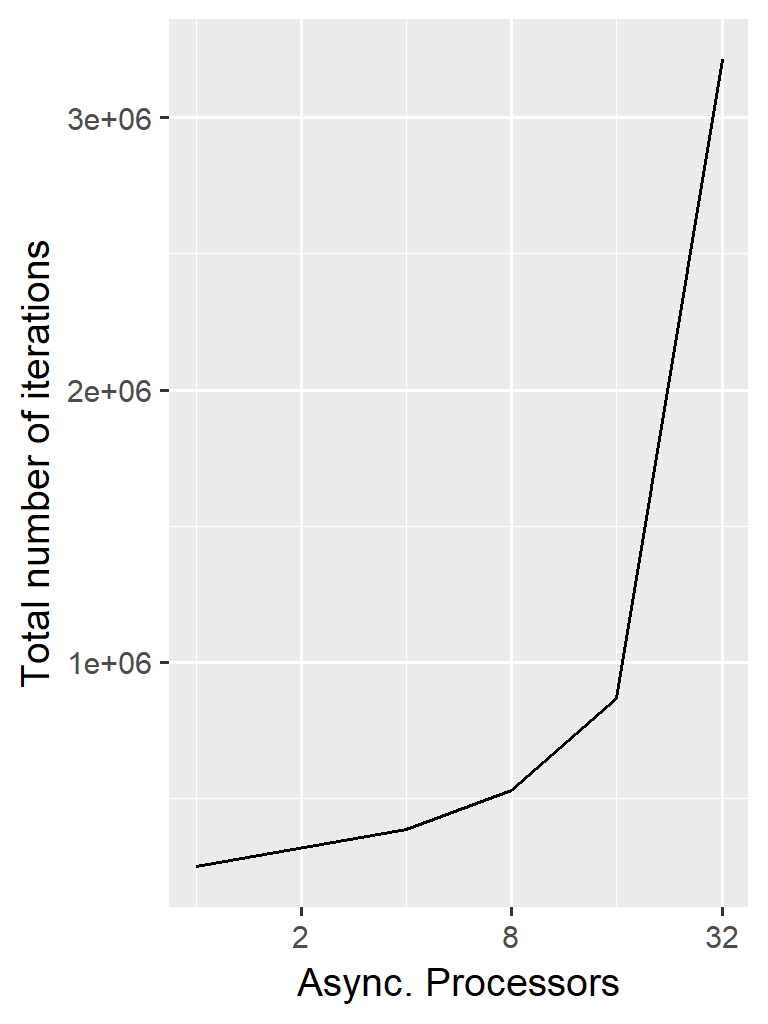
\includegraphics[width=1.0\linewidth]{./chapters/05.pcdm/scalability/speedup_pcdm_iter.png}
	\end{subfigure}
	\begin{subfigure}{0.30\linewidth}
		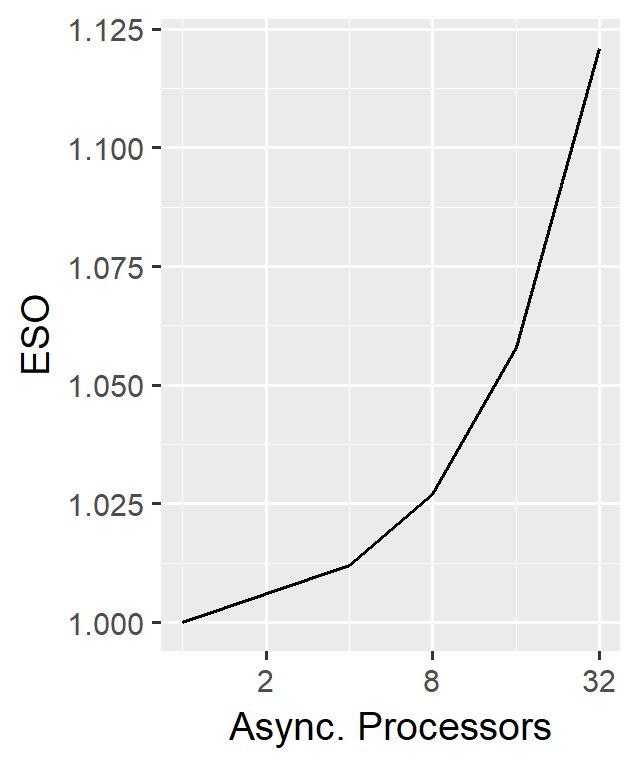
\includegraphics[width=1.0\linewidth]{./chapters/05.pcdm/scalability/speedup_pcdm_eso.png}
	\end{subfigure}
	\caption{Speedup comparison with increasing number of asynchronous processors.}
	\label{pcdm:scalability:proc}
\end{figure}

We see a linear speedup up to 8 processors. But afterwards, the speedup we receive diminishes quickly. After 16 processors, the parallel coordinate descent algorithm even becomes slower when more processors are added. The reason for this behavior lies in the total number of iterations the parallel algorithm needs to reconstruct a solution. As we see in Figure \ref{pcdm:scalability:proc} needs over 3 million parallel iterations to converge with 32 asynchronous processors. With 8 processors, it about half a million iterations to converge.

This drastic increase in total iterations quickly diminishes the speedup we receive by adding more asynchronous processors. This is partly due to the increase in the ESO: Adding more asynchronous processors increases the ESO, which in turn reduces the step size by which we can minimize a pixel in each iteration. However, we suspect there are more effects at play than just the ESO. The ESO for the number of processors is also shown in Figure \ref{pcdm:scalability:proc} does not increase as drastic as the total number of iterations needed. 

\begin{table} [h]
	\centering
		\begin{tabular}{c | r }
			Processors & Iterations per second \\ \hline
			1 & 1061.7 \\
			4 & 3849.7 \\
			8 & 9254.9 \\
			16 & 16'721.9 \\
			32 & 32'794.6 \\
		\end{tabular}
	\caption{Throughput of the parallel coordinate descent algorithms with additional processors.}
	\label{pcdm:scalability:throughput}
\end{table}

When we look at the throughput of the parallel coordinate descent algorithm in table \ref{pcdm:scalability:throughput}, we see that the number of iterations per second still increases roughly linearly with the number of asynchronous processors. If the parallel algorithm gets slowed down because of communication costs between processors (for example: multiple compare-exchange operations on the same entry in the gradient map), we would see a less-than-linear increase in throughput per added processor. Meaning the slowdown we see in Figure \ref{pcdm:scalability:proc} is likely not due to communication costs, but due to the drastic increase in total number of iterations.

Remember that the parallel coordinate descent algorithm uses active set iterations: Each asynchronous processor chooses pixels from the active set for a given number of iterations. When we measure the absolute maximum pixel difference (the maximum step a serial greedy coordinate descent algorithm can take in one iteration) for 8 processors, we observe that it steadily decreases from one active set iteration to the next. At 32 processors, the absolute maximum pixel difference fluctuates from one active set iteration to the next.

This observation leads us to the ESO and our pseudo-random selection strategy: We may see the fluctuation, because we do not choose pixels uniformly at random, and their $PSF$s overlap more than we estimated with the ESO. In that case, the algorithm is in the danger of diverging, which would explain the fluctuation. The solution in that case would be to increase the ESO.

On the other hand, this fluctuation can also be observed with a proper random selection strategy. The second explanation is that with increasing number of processors, a single processor is simply too close to a random selection strategy. Remember: Our pseudo-random strategy greedily searches a fraction of the active set. With an active set of 1024 entries, 32 processors and a search fraction of 0.1, each processor searches 10\% of $\frac{1024}{32}$ entries. By adding more processors, each processor searches through fewer entries, although the total number of entries searched stays the same. The solution in that case would be to increase the Search Fraction.

We tested these two explanations: We ran the parallel coordinate descent algorithm once with an increased ESO (the ESO which arises from 64 processors) and once with an increased Search Fraction. The results are summarized in Table \ref{pcdm:scalability:table}.

\begin{table} [h]
	\centering
	\begin{tabular}{c | r | r | r | r | r | c}
		Test & Processors &  ESO & Search Fraction & \# Iterations & Total Seconds & Speedup\\ \hline \hline
		Standard & 16 & 1.058 & 0.1 &  868k & 51 & 4.5\\\hline
		Standard & 32 & 1.121 & 0.1 & 3'213k & 98 & 2.4\\
		Larger ESO & 32 &  1.246 & 0.1 & 4'220k & 130 & 1.8 \\
		Larger Search & 32 &  1.121 & 0.4 & 1'171k & 47 & \textbf{5.0} \\
	\end{tabular}
	\caption{Speedup comparison for the parallel coordinate descent algorithm, once with increased ESO and once with increased Search Fraction.}
	\label{pcdm:scalability:table}
\end{table}

Increasing the Search Fraction lead to a significant decrease in total iterations, which in turn leads to a significant decrease in the wall-clock time, leading to a speedup factor of 5. This means, with a larger Search Factor, the parallel coordinate descent algorithm is again faster with 32 processors instead of 16, and it would remove the 'dip' in Figure \ref{pcdm:scalability:proc}. Noteworthy is that increasing the ESO in our parallel algorithm again lead to an increase in total number of iterations. This result suggests the ESO was not too low, and was not at fault for the slowdown we measured in Figure \ref{pcdm:scalability:proc}. 

Nevertheless, these results are still surprising to us. As we mentioned before, whether we use 1 processor or 16 in our parallel coordinate descent algorithm, we still search the same number of elements in the active set. For a Search Fraction of 0.1, the algorithm always searches 10\% for every parallel iteration. Adding more processors simply reduces the number of elements each processor checks. The results from Table \ref{pcdm:scalability:table} suggests that each processor in our parallel algorithm has to search through a minimum number of elements in the active set to run efficiently. But this view does not agree with our results from Figure \ref{pcdm:results:search}, where we used 8 processors and a Search Fraction of 0.01. Each of the 8 processors searched through fewer elements than in this test with 32 processors and a Search Fraction of 0.1. But with 8 processors, it did not lead to a large increase in wall-clock time.

It is not clear why exactly our parallel coordinate descent algorithm needs so many more iterations to converge with 32 processors, or why increasing the Search Fraction can remedy the problem. But the total number of iterations needed to converge seem to be the bottleneck for this algorithm. A thorough analysis may lead to a variant of our algorithm which needs fewer iterations to converge and therefore may be even faster. In the time frame of this project, it was not possible to further analyze the behavior.